%% ------ Packages ------ %%
% Related to the document setup:
\documentclass[12pt, a4paper]{extarticle}
\usepackage[a4paper, top = 2.4cm, bottom = 2.4 cm, right= 2.1cm, left= 2.1cm]{geometry}
\usepackage[english]{babel}
\renewcommand\familydefault{\sfdefault}
\usepackage{lmodern}
\usepackage{amsmath}
\usepackage{mathtools}
\usepackage{amsfonts}
\usepackage{amssymb}

\usepackage[T1]{fontenc}
\setlength\parindent{0pt}
\usepackage{multicol}
\usepackage{xspace}

\usepackage{tocloft}

% Colouring the references
\usepackage{hyperref}
\usepackage{cleveref}
\usepackage[dvipsnames]{xcolor}
\pagecolor{white}
\newcommand\myshade{85}
\colorlet{mylinkcolor}{violet}
\colorlet{mycitecolor}{YellowOrange}
\definecolor{myurlcolor}{rgb}{ 0, 0.4470, 0.6410}

\hypersetup{
  linkcolor  = mylinkcolor!\myshade!black,
  citecolor  = mycitecolor!\myshade!black,
  urlcolor   = myurlcolor!\myshade!black,
  colorlinks = true,
}

% Nomenclature
%\usepackage{nomencl}
%\makenomenclature
%%\renewcommand{\nomname}{List of symbols}
%\renewcommand{\nompreamble}{\noindent Definitions of the nomenclature}
%\newlength{\nomitemorigsep}
%\setlength{\nomitemorigsep}{\nomitemsep}
%\setlength{\nomitemsep}{-\itemsep}

% Section properties redefinitions
\makeatletter
\renewcommand\section{\@startsection {section}{1}{\z@}{3ex }{0.7ex } {\normalfont\large\bfseries}}
\renewcommand\subsection{\@startsection{subsection}{1}{\z@}{2ex }{0.1ex } {\normalfont \bfseries}}
\renewcommand\subsubsection{\@startsection{subsubsection}{3}{\z@}{-1.5ex\@plus -1ex \@minus -.2ex}{.5ex}{\normalfont}}
\makeatother

% Graphics interfaces:
\usepackage{graphicx}
\usepackage{tikz}
\tikzset{every picture/.style={line width=1pt}}
\usepackage{float}
\usepackage{subcaption} 
\usepackage[font=small,aboveskip=3pt, belowskip=-0pt]{caption}


% Headers and footers:
\usepackage{url}
\usepackage{footnote}
\usepackage{fancyhdr}
\pagestyle{fancy} 
\fancyhf{} 
\renewcommand{\headrulewidth}{0pt}
\newcommand{\mainmatter}{\clearpage \cfoot{\thepage\ of \pageref{LastPage}}
\setcounter{page}{1}
\pagenumbering{arabic}}
%\usepackage{comment}

\lfoot{\footnotesize \textcolor{Gray}{\thesistitle.}}
\rfoot{\footnotesize \textcolor{Gray}{\thesisauthor, \studentnumber. \thedate.}}
\fancyhfoffset{0pt}


% Sort the bibliography and add to the table of contents
\usepackage[sort]{cite}
\setlength\columnsep{15pt}
\usepackage[nottoc,numbib]{tocbibind}

% Redefine the \left and \right operators:
\let\originalleft\left
\let\originalright\right
\renewcommand{\left}{\mathopen{}\mathclose\bgroup\originalleft}
\renewcommand{\right}{\aftergroup\egroup\originalright}

% Redefine \eqref environment
\usepackage{letltxmacro}
\LetLtxMacro{\originaleqref}{\eqref}
\renewcommand{\eqref}{Equation~\originaleqref}

% Command definitions and macros:
\newcommand{\ic}{{\rm{i}}\xspace}
\renewcommand{\Re}{{\operatorname{Re}}\xspace}
\renewcommand{\Im}{{\operatorname{Im}}\xspace}

\newcommand{\Pulse}{{\mathcal{P}}\xspace}
\newcommand{\kmean}{{\langle k\rangle}\xspace}
\renewcommand{\k}{{\boldsymbol{k}}\xspace}
\newcommand{\kacc}{{\boldsymbol{k'}}\xspace}
\newcommand{\kin}{{k^{\rm in}}\xspace}
\newcommand{\kout}{{k^{\rm out}}\xspace}
\newcommand{\kinb}{{\boldsymbol{k^{\rm in}}}}
\newcommand{\koutb}{\boldsymbol{{k^{\rm out}}}}
\newcommand{\kinbi}{{\boldsymbol{k}_i^{\bf in}}}
\newcommand{\koutbj}{{\boldsymbol{k}_j^{\bf out}}}
\newcommand{\degree}{{\rm deg}\xspace}
\newcommand{\kmin}{k_{\text{min}}\xspace}
\newcommand{\kmax}{k_{\text{max}}\xspace}

\newcommand{\Sin}{{S^{\rm in}}\xspace}
\newcommand{\Sout}{{S^{\rm out}}\xspace}

\newcommand{\dtheta}{{\dot{\theta}}\xspace}

\newcommand{\permute}{{\digamma}\xspace}
\newcommand{\permuteinv}{{\digamma^{-1}}\xspace}

%\newcommand{\R}{{\rm I\!R}\xspace}
\newcommand{\R}{{\mathbb{R}}\xspace}
\renewcommand{\c}{{\mathbb{C}}\xspace}
\newcommand{\C}{\mathbb{C}_\circ}
\newcommand{\T}{{\mathbb{T}}\xspace}
\newcommand{\K}{{\mathbb{K}}\xspace}

\newcommand{\tp}{{t^{\prime}}\xspace}
\newcommand{\tpp}{{t^{\prime \prime}}\xspace}

\newcommand{\QIF}{{\textsl{QIF}}\xspace}
\newcommand{\PRC}{{\textsl{PRC}}\xspace}
\newcommand{\pdf}{{\textsl{pdf}}\xspace}
\newcommand{\MFR}{{\textsl{MFR}}\xspace}
\newcommand{\SNIC}{{\textsl{SNIC}}\xspace}
\newcommand{\PSR}{{\textsl{PSR}}\xspace}
\newcommand{\PSS}{{\textsl{PSS}}\xspace}
\newcommand{\CPW}{{\textsl{CPW}}\xspace}
\newcommand{\STDP}{{\textsl{STDP}}\xspace}
\newcommand{\ISI}{{\textsl{ISI}}\xspace}
\newcommand{\IP}{{\textsl{IP}}\xspace}



\def\matlab{\textsc{Matlab}\xspace}

% Author macros:
\newcommand{\thesistitle}{The dynamics of adaptive neuronal networks}
\newcommand{\thesissubtitle}{influence of topology on synchronisation }
\newcommand{\mywork}{{\textsl{Investigation:}}\xspace}

\newcommand{\thesisauthor}{Simon Aertssen} % Your name :) 
\newcommand{\studentnumber}{s181603}
\newcommand{\thedate}{February 1$^{\text{st}}$ 2021} 
\newcommand{\thesissupervisorI}{Erik Martens} 
\newcommand{\thesissupervisorII}{Poul Hjorth} 

\newcommand{\department}{DTU Compute}
\newcommand{\departmentdescriber}{Department of Applied Mathematics and Computer Science}
\newcommand{\addressI}{Richard Petersens Plads, Building 324}
\newcommand{\addressII}{2800 Kgs. Lyngby, DK}
\newcommand{\departmentwebsite}{www.compute.dtu.dk}


%% ------ Front page ------ %%

\begin{document}

\mainmatter

Status meeting \today \\
Msc Thesis - Dynamics of adaptive neuronal networks. \\
Simon Aertssen (s181603), \today \\ 

\section{Writing out the whole system}
The network dynamics are described as follows:
\begin{align}
\frac{d \theta_i}{d t} &= (1 - \cos\theta_i) + (1 + \cos\theta_i)\cdot\left(\eta_i + I_i \right) \nonumber \\
I_{i} &= \frac{\kappa}{\langle k\rangle} \sum_{j=1}^{N} A_{i j} P_{n}\left(\theta_{j}\right) \label{eq:FullThetaNeuronNetwork} \\
P_{n}\left(\theta_{j}\right) &= (1 - \cos\theta_j) \nonumber
\end{align}

We observe synchronization through the order parameter
\begin{align}
Z(t) = \frac{1}{N} \sum_{j=1}^N e^{\ic\theta(t)_j} \label{eq:orderparameter}
\end{align}

For a fixed degree network it has been proven that the order parameter follows:
\begin{align}
\dot{Z}(t)= -\ic \frac{(Z-1)^2}{2}+\frac{(Z+1)^2}{2} \cdot \left(-\Delta+ \ic\eta_{0}
+ \ic \kappa \cdot \left(1+\frac{Z^{2} + \overline{Z}^{2} }{6} - \frac{4}{3} \Re(Z)\right)\right) \label{eq:MeanField}
\end{align}
    
For an arbitrary network the order parameter follows a trajectory per degree. When we assemble the whole expression for the Ott-Antonsen manifold as found in \cite{OttAntonsen2017} with $H_2(\k,t)$ as in \cite{Martens2020}, we obtain the following:
\begin{align}
\frac{\partial z(\k, t)}{\partial t} &= -\ic \frac{(z(\k, t)-1)^{2}}{2} + \frac{(z(\k, t)+1)^{2}}{2} \cdot I(\k) \nonumber \\
I(\k) &= -\Delta(\k) + \ic \eta_{0}(\k) + i d_{n} \kappa \cdot H_n(\k,t) \label{eq:OttAntonsenSystemFull} \\
%H_n(\k,t) &= \frac{a_n}{\kmean} \sum_{\kacc} P\left(\kacc\right) a\left(\kacc \rightarrow \k\right) \cdot \left[A_{0}+\sum_{p=1}^{n} A_{p}\left(z\left(\kacc, t\right)^{p} + \overline{z}\left(\kacc, t\right)^{p}\right)\right] 
H_2(\k,t) &= \frac{1}{\kmean} \sum_{\kacc} P\left(\kacc\right) a\left(\kacc \rightarrow \k\right) \cdot \left( 1 + \frac{z(\kacc, t)^2 + \overline{z}(\kacc, t)^2}{6} - \frac{4}{3} \Re(z(\kacc, t)) \right) \nonumber
\end{align}

We can then find the mean field dynamics through
\begin{align}
\overline{Z}(t) &= \frac{1}{N} \sum_{\k} P(\k) z(\k, t) \label{eq:OttAntonsenMeanField}
\end{align}

It is important to notice that in \eqref{eq:OttAntonsenSystemFull} and \eqref{eq:OttAntonsenMeanField} we actually compute an inner vector product, which is non-commutative for complex numbers:
\begin{align}
a \cdot b = \overline{b \cdot a} \quad a, b \in \C^r
\end{align}
This is the result of the \textsl{Conjugate} or \textsl{Hermitian} symmetry of the inner product.


\section{Initial conditions}
As the systems in \cref{eq:FullThetaNeuronNetwork,eq:orderparameter,eq:MeanField,eq:OttAntonsenSystemFull,eq:OttAntonsenMeanField} describe the same dynamics for fully connected networks, it is important to be able to transform initial conditions between systems.
\begin{align}
\end{align}

\section{Fixpoint iteration}
In \cite{OttAntonsen2017} a fixpoint iteration is suggested to find attractive fixpoints of the system \eqref{eq:OttAntonsenSystemFull}. If we set $\frac{\partial z(\k, t)}{\partial t} = 0$ we can solve the following system:
\begin{align}
\ic \frac{(z(\k, t)-1)^{2}}{2} &= \frac{(z(\k, t)+1)^{2}}{2} \cdot I(\k) \nonumber \\
\ic \left(\frac{z(\k, t)-1}{z(\k, t)+1}\right)^2 &= I(\k) \nonumber \\
\frac{z(\k, t)-1}{z(\k, t)+1} &\equiv b(\k,t) \nonumber \\
z(\k, t) - 1 &= b(\k,t) z(\k, t) + b(\k,t)  \nonumber \\
z(\k, t) \cdot (1 - b(\k,t)) &= b(\k,t)  + 1\nonumber
\end{align}

We can then obtain the stable equilibria from:
\begin{align}
\ic b(\k,t)^2 = I(\k) \hspace{10mm} z(\k, t)_{\pm} = \frac{1 \pm b(\k,t)}{1 \mp b(\k,t)} \label{eq:fixedpointiterations} 
\end{align}
where the signs are chosen so that $\vert z(\k, t) \vert \leq 1$.


\section{A Newton-Raphson iteration for all fixpoints}
\subsection{Theory behind the method}
The fixpoint iteration only gives us the stable equilibria of the system \eqref{eq:OttAntonsenSystemFull}. We can obtain all equilibria and the Jacobian from a Newton-Raphson iteration. We define the equilibria $\boldsymbol{x^\ast} \in \R^n$ of a multivariate function $\boldsymbol{f}(\boldsymbol{x}) : \R^n \rightarrow \R^n$ with $\boldsymbol{f}(\boldsymbol{x}) = \boldsymbol{0}$. Expanding $\boldsymbol{f}$ as a Taylor series, we obtain:
\begin{align}
f_i(\boldsymbol{x} + \delta \boldsymbol{x}) =f_{i}(\boldsymbol{x}) + \sum_{j=1}^{n} \frac{\partial f_{i}(\boldsymbol{x})}{\partial x_{j}} \delta x_{j}+O\left(\delta \boldsymbol{x}^{2}\right) \approx f_{i}(\boldsymbol{x})+\sum_{j=1}^{n} \frac{\partial f_{i}(\boldsymbol{x})}{\partial x_{j}} \delta x_{j}, \quad(i=1, \cdots, n)
\end{align}

We can also write this in vector notation, by setting $\boldsymbol{J}(\boldsymbol{x}) = \nabla \boldsymbol{f}(\boldsymbol{x}) = \frac{d}{d\boldsymbol{x}} \boldsymbol{f}(\boldsymbol{x}) \in \R^{n \times n}$ 
\begin{align}
\boldsymbol{f}(\boldsymbol{x}+\delta \boldsymbol{x}) &\approx\left[\begin{array}{c}f_{1}(\boldsymbol{x}) \\ \vdots \\ f_{N}(\boldsymbol{x})\end{array}\right] 
+ \left[\begin{array}{ccc}\frac{\partial f_{1}}{\partial x_{1}} & \cdots & \frac{\partial f_{1}}{\partial x_{N}} \\ \vdots & \ddots & \vdots \\ \frac{\partial f_{N}}{\partial x_{1}} & \cdots & \frac{\partial f_{N}}{\partial x_{N}}\end{array}\right]
\left[\begin{array}{c}\delta x_{1} \\ \vdots \\ \delta x_{N}\end{array}\right] 
=\boldsymbol{f}(\boldsymbol{x})+\boldsymbol{J}(\boldsymbol{x}) \delta \boldsymbol{x} 
\end{align}

By assuming $\boldsymbol{f}(\boldsymbol{x}+\delta \boldsymbol{x}) = 0$ we can find that $\delta \boldsymbol{x} = -\boldsymbol{J}^{-1}( \boldsymbol{x}) \boldsymbol{f}(\boldsymbol{x})$ so that $\boldsymbol{x} + \delta \boldsymbol{x} =  \boldsymbol{x} - \boldsymbol{J}^{-1} (\boldsymbol{x}) \boldsymbol{f}(\boldsymbol{x})$. This expression converges to $\boldsymbol{x^\ast}$. When the equations are nonlinear, the equations converge to the real root as $\boldsymbol{x}_k =  \boldsymbol{x}_k - \boldsymbol{J}^{-1} ( \boldsymbol{x}_k)\boldsymbol{f}(\boldsymbol{x}_k)$. \\

For \eqref{eq:OttAntonsenSystemFull}, we can compute the Jacobian for the diagonal and off-diagonal elements separately. But as $z(\k,t)$ is a complex function, first we need to understand what the derivative of a complex function is. 


\subsection{Derivatives of complex functions}
For $z = x + \ic y \in \C$ and $x,y \in R$ the conjugate is defined as $\overline{z} = x - \ic y$. That means that we can write the real and imaginary parts as:
\begin{align*}
x = \frac{z + \overline{z}}{2} \text{  and   }   y = -\ic \frac{z - \overline{z}}{2}
\end{align*}
Using the chain rule, we can write the partial derivative with respect to $z$ in function of $x$ and $y$ as $x$ and $y$ are functionally independent and find the first Wirtinger operator:
\begin{align*}
\frac{\partial}{\partial z} =\frac{\partial x}{\partial z} \frac{\partial}{\partial x}+\frac{\partial \bar{y}}{\partial z} \frac{\partial}{\partial \overline{y}} 
\longrightarrow \frac{\partial x}{\partial z} = \frac{1}{2} \text{   and   } \frac{\partial y}{\partial z} =  - \frac{\ic}{2} 
\longrightarrow \frac{\partial}{\partial z} = \frac{1}{2}\left(\frac{\partial}{\partial x} - \ic \frac{\partial}{\partial y}\right)
\end{align*}
We note the following properties:
\begin{align*}
\frac{\partial}{\partial z} z = 1 \hspace{10mm} \frac{\partial}{\partial z}\overline{z} = \frac{1}{2}\left(1 - \ic^2 \right) = 0
\end{align*}
Interesting for is the result of the following: 
\begin{align*}
\overline{z}^2 &= (x - \ic y)^2 = x^2 - y^2 - \ic 2xy \\
\frac{\partial}{\partial z} \overline{z}^2 &=  \frac{1}{2}\cdot(2x -\ic 2y - \ic\cdot(-2y -\ic 2x)) = x -\ic y + \ic y -\ic x = 0
\end{align*}



\subsection{Derivatives of the complex mean field equations}
We can now compute derivatives of the complex functions $z(\k,t)$. When setting $z(\k, t) = z_k$ the diagonal elements are found as
\begin{equation}
\begin{aligned}[b]
\frac{\partial}{\partial z_k}\left(\frac{\partial z_k}{\partial t} \right) &= - \ic(z_k - 1) + (z_k + 1) \cdot I(z_k) +  \frac{(z_k+1)^{2}}{2} \cdot \frac{\partial I(z_k)}{\partial z_k} \\
\frac{\partial I(z_k)}{\partial z_k} &= \ic \kappa \cdot \frac{\partial H_{2,k}}{\partial z_k} \\
\frac{\partial H_{2,k}}{\partial z_k} &= \frac{1}{\kmean} P_k a_{kk} \cdot \left(\frac{2 z_k}{6} - \frac{4}{3} \cdot \frac{1}{2} \right) = \frac{1}{\kmean} P_k a_{kk} \cdot\frac{z_{k} - 2}{3}
\end{aligned}
\label{eq:OttAntonsenSystemJacobianDiagonal}
\end{equation}

When setting $z(\kacc, t) = z_{k'}$ the off-diagonal elements are found as
\begin{equation}
\begin{aligned}[b]
\frac{\partial}{\partial z_{k'}}\left(\frac{\partial z_k}{\partial t} \right) &= \frac{(z_k + 1)^{2}}{2} \cdot \frac{\partial I(z_k)}{\partial z_{k'}} \\
\frac{\partial I(z_k)}{\partial z_{k'}} &= \ic \kappa \cdot \frac{\partial H_{2,k}}{\partial z_{k'}} \\
\frac{\partial H_{2,k}}{\partial z_{k'}} &= \frac{1}{\kmean} P_{k'} a_{k'k} \cdot \frac{z_{k'} - 2}{3}
\end{aligned}
\label{eq:OttAntonsenSystemJacobianDiagonal}
\end{equation}


\subsection{Results}
I cannot seem to converge close enough.
\begin{figure}[H]
\centering
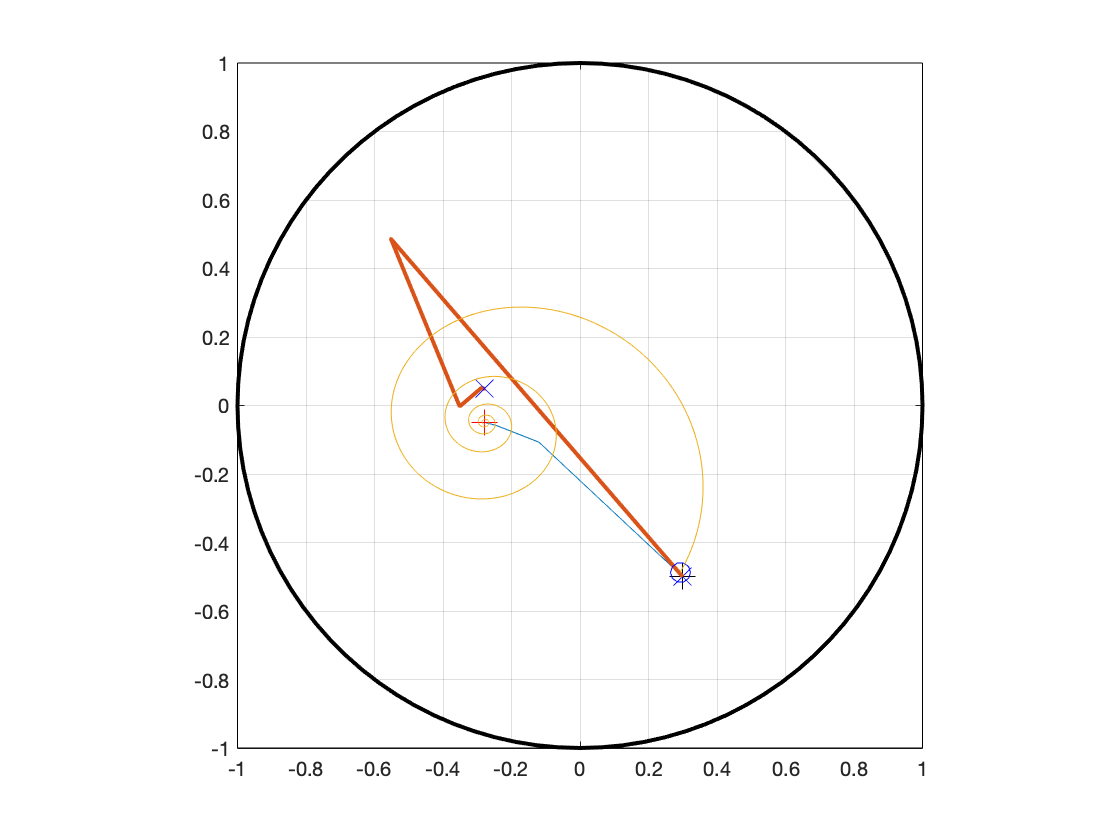
\includegraphics[width = \textwidth]{../Figures/ProblemsWithNewtonRaphson.png}
\end{figure}



\bibliographystyle{utphys}
\small{\bibliography{references}}

\label{LastPage}~

\end{document}
